%%%%%%%% Sample LaTeX input for Complex Systems %%%%%%%%%%% 
% Revision 4, Jun 27, 2018
%
% This is a LaTeX input file  
% Text following % on a particular line is treated as a comment, and 
% ignored by LaTeX.  
% You do not need to type any text that follows a % 
% 
\documentclass{article}

\usepackage{graphicx,hyperref}
\usepackage{amssymb,ComplexSystems}
\usepackage{tikz}
\usetikzlibrary{automata, positioning, arrows}
\graphicspath{ {./images/} }

% complex-systems.sty is the macro package for Complex Systems.
% It is available at
% http://www.complex-systems.com/samples/complex-systems.sty
% epsf.sty is the preferred graphics import method

\begin{document}

\title{Relazione di Progetto - Reti Logiche% 
% Use \\ to indicate line breaks in titles longer than about 
% 55 characters. 
%
}

\author{\authname{Elia Maggioni}\\[2pt] 
% Use \\[2pt] to end the line and add space between author name and affiliation. 
\authadd{Ingegneria Informatica, Scuola 3I, Polimi}\\
\authadd{C.P. 10610008}\\
\and
% For extra space, precede the second set of authors with \and.
\authname{Marco Fasanella}\\
\authadd{Ingegneria Informatica, Scuola 3I, Polimi}\\
\authadd{C.P. 10617541}\\
% Do not use a ``.'' at the end of any line in the address. 
}

% The following specifies the running headings 
%
% Each running heading should be less than about 50 characters long. 
% If necessary, give a shortened version of the title. 
%
% Use initials for first and second names. If all author names do not fit, truncate the 
% list and end with ``et al.''.
\markboth{Progetto di Reti Logiche} 
{Relazione di Progetto} 

\maketitle
% End title section

\begin{abstract}
Nel progetto abbiamo seguito un approccio top-down partendo dal disegno su carta delle FSM e dei DataPath, traduzione in codice VHDL, testing generico e testing mirato agli edge-case.
\end{abstract}

% The text of the paper follows. All of the text should be in the same file. 
% Use separate files for large tabular material and graphics.

\section{Introduzione}
\label{intro}
% \label is a hyperlink target for cross-referencing to this section using \ref{intro} (optional).
Il circuito descritto si occupa di leggere e rielaborare i dati da RAM producendo un'immagine con nitidezza più alta e quindi più leggibile. 
Quando il segnale start è fornito al circuito, viene attivata la prima macchina a stati ed in base al bias tra la saturazione dei pixel e l'offset, ovvero il valore minimo di saturazione, viene restituita nei valori di memoria immediatamente successivi un'immagine che meglio ricopre la gamma di colore rappresentabile.
Quando la elaborazione è terminata, viene restituito un segnale di done ed il circuito è pronto per una nuova immagine a partire dall'indirizzo 0.

Nel circuito è stato scelto di dividere in 3 la computazione con moduli in cascata.

\begin{figure}[h]
\centering

\includegraphics[width=0.7\textwidth]{introduzioneimg1.png}
\caption{Example of a parametric plot}
\end{figure}
\break

\section{Architettura}

La scelta architetturale ricade sull'utilizzo di 3 moduli, descritti ognuno da una propria FSM, attraverso segnali in cascata per l'avvio e la terminazione delle varie parti. Si avranno quindi i segnali start2,start3,done2, e done3 che avranno come scopo la comunicazione fra i vari moduli e i loro processi.
 \begin{enumerate} 
  \item \textbf{Modulo 1} 
  
  Il primo modulo si occupa dell'inizio della computazione, della lettura e ricerca di massimo, minimo, e delta. Inoltre attende la discesa del segnale start in modo da abbassare done e mettersi in attesa di una nuova immagine. La macchina a stati di riferimento (FSM1) è composta dai seguenti stati:
  \begin{itemize}
  \item F1S0
  
  Stato iniziale che attende il segnale di start. Si entra in questo stato per azzerare i registri e prepararsi a processare l'immagine.
  
    \item F1S1,F1S2,F1S1b,F1S2b
  
  Questi stati si occupano della lettura di OP1 e OP2 (numero righe e colonne) attraverso il processo MULT. In F1S2b un controllo si accerterà che OP1 non sia nullo, altrimenti si passerà allo stato di terminazione e reset dei valori per una nuova lettura.
  \item F1S3,F1S3b
  
  A questo punto viene calcolato M (cioè \(OP1*OP2\)) facendo rimbalzare questi due stati attraverso il segnale o-m. Il calcolo avviene per somme successive fino a quando OP2 sarà zero. 
  \item F1S4,F1S4a,F1S5
  
  Attraverso i processi ADDRHandler e MINeMAX, verrà incrementato REGAddr (registro dell'indirizzo di memoria) e controllato Pixel (registro che salva ogni current pixel). Il segnale f1 detta il passaggio fra questi stati attraverso la condizione \(REGAddr > M + 2 \). Il calcolo del delta invece, avviene ad ogni nuovo assegnamento del Massimo o del Minimo.
  
  \item F1S6,F1S7
  
  Una volta terminato il proprio compito, nello stato F1S6 verrà alzato il segnale start2 per far partire il secondo modulo e successivamente, lo stato F1S7 si metterà quindi in attesa del segnale done2 per terminare l'elaborazione e reset dei valori.
  \item F1S8,F1S9
  
  A questo punto, una volta ricevuto il segnale done2, lo stato F1S8 alzerà done ed endof (segnale generale di imminente terminazione e reset dei valori), e aspetterà che si abbassi start, per poi passare a F1S9 che farà riscendere i due precedenti segnali. Si torna quindi a F1S0 in attesa di una nuova immagine.
\end{itemize}
\begin {center}  
	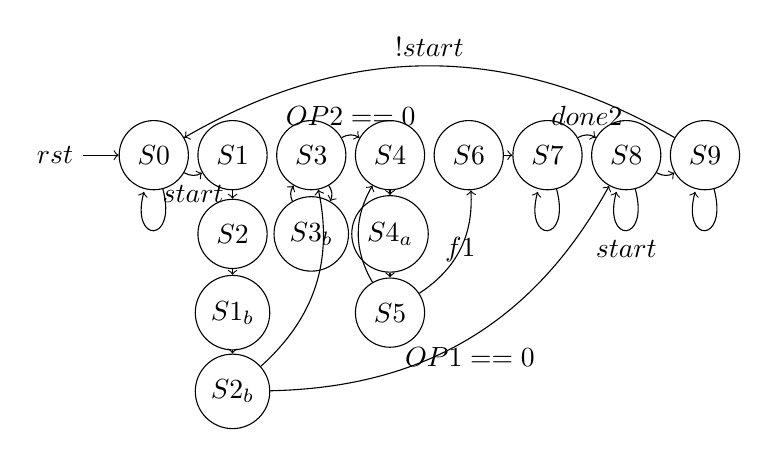
\begin{tikzpicture}
	[->,align=center,node distance=1cm]
    \node[state,initial,initial where=left, initial text=$rst$] (S0) {$S0$};
    \node[state, right of=S0] (S1) {$S1$};
    \node[state, below of=S1] (S2) {$S2$};
    \node[state, below of=S2] (S1b) {$S1_b$};
    \node[state, below of=S1b] (S2b) {$S2_b$};
      \node[state, right of=S1] (S3) {$S3$};
      \node[state, below of=S3] (S3b) {$S3_b$};
       \node[state, right of=S3] (S4) {$S4$};
      \node[state, below of=S4] (S4a) {$S4_a$};
      \node[state, below of=S4a] (S5) {$S5$};
      \node[state, right of=S4] (S6) {$S6$};
      \node[state, right of=S6] (S7) {$S7$};
      \node[state, right of=S7] (S8) {$S8$};
      \node[state, right of=S8] (S9) {$S9$};
       \draw   (S0) edge[bend right,below] node{$start$} (S1)
       (S0) edge[loop below] node{} (S1)
            (S1) edge[ below] node{} (S2)
            (S2) edge[ below] node{} (S1b)
            (S1b) edge[ below] node{} (S2b)
            (S2b) edge[ bend right,below ] node{$OP1==0$} (S8)
            (S2b) edge[ bend right] node{} (S3)
            (S3) edge[ bend left, above] node{} (S3b)
            (S3) edge[ bend left, above] node{$OP2==0$} (S4)
            (S3b) edge[ bend left] node{} (S3)
            (S4) edge[ below] node{} (S4a)
            (S4a) edge[ below] node{} (S5)
            (S5) edge[ bend left] node{} (S4)
            (S5) edge[ bend right] node{$f1$} (S6)
            (S6) edge[ right] node{} (S7)
              (S7) edge[ loop below] node{} (S7)
                (S8) edge[ loop below] node{$start$} (S8)
                (S9) edge[ loop below] node{} (S9)
            (S7) edge[ bend left,above] node{$done2$} (S8)
            (S8) edge[ bend right,below] node{} (S9)
            (S9) edge[bend right,above] node{$!start$} (S0);
\end{tikzpicture}
\end{center}  
  
    \item \textbf{Modulo 2}
		
		Il modulo due svolge il calcolo dello shift level noto il data value e lo rende disponibile per l'utilizzo al modulo tre. Una volta completato il calcolo, alza il segnale start3 per fare partire la FSM3 ed attende il done3 prima di terminare dando il done2 al modulo uno. Di seguito la descrizione della FSM2 che ha quasi solo una funzione di timing dei registri:
			\begin{itemize}
				\item F2S0 
				
				Attende l'inizio dell'esecuzione del programma che avviene tramite l'innalzamento del segnale start2
				
				\item F2S1
				
				Carica il valore di delta nel registro S2R1
				
				\item F2S2,F2S3,F2S4
				
				Attende la propagazione del segnale nel datapath e carica il valore in uscita dalla LUT in S2R2
				
				\item F2S5
				
				Avvia il modulo tre alzando il segnale start3
				
				\item F2S6
				
				Attende in questo stato finché done3 non viene alzato dal modulo tre
				\item F2S7
				
				Alza il done2 per segnalare al modulo due l'avvenuta terminazione dell'elaborazione.
				
				
			\end{itemize}
    \item\textbf{Modulo 3} 
		
		Il modulo tre è dove avviene la parte più delicata dell'elaborazione, in particolare a questa parte è delegata la lettura da memoria del valore del pixel corrente, il calcolo sequenziale per ogni pixel del nuovo valore e la riscrittura in memoria.
		
		\begin{itemize}
		
		\item F3S0
		
		Stato di attesa della macchina, passa a \emph{F3S0b} quando start3 è portato a 1
		
		\item F3S0b, F3S0c
		
		In questi due stati viene prelevato da memoria il valore corrente del pixel ed assegnato al registro \emph{F3R3} che simboleggia il \emph{CurrPixel} value. La gestione della memoria viene effettuata tramite i flag \emph{o\_f3addr\_read \emph{e} o\_f3addr\_write} in un processo separato. Viene quindi assegnato il valore di ritorno \emph{i\_data}.
		
		\item F3S1
		
		Avviene ora il prelievo dei segnali provenienti dai moduli uno e due e il caricamento degli stessi nei registri \emph{F3R1}, \emph{F3R2} e \emph{F3R4}, rispettivamente \textit{Shift\_level, min pixel value \emph{e} max address}.
		
		\item F3S2, F3S3
		
		In questi stati avviene il calcolo di \(CurrPixel - minV\) e viene propagato tramite il segnale \emph{o\_f3sub} che poi viene caricato in \emph{F3R5}
		
		\item F3S4
		
		Da \emph{shift\_level} e \emph{F3R5} viene calcolato il valore di \emph{o\_f3shift}, vettore di 16 bit per evitare il possibile overflow
		
		\item F3S5, F3S6
		
		Un mutex viene inserito per portare \emph{shift\_level} da 16 bit a 8, nel caso in cui sia minore di 255 gli 8 bit più significativi vengono scartati, altrimenti viene assegnato il valore massimo rappresentabile di 255.
		
		\item F3S6b, F3S7
		
		Tramite il flag \emph{o\_f3addr\_write} viene assegnato in \emph{o\_data} il valore finale del registro \emph{F3R6} in uscita al mutex.
		
		\item F3S7b, F3S8
		
		Il valore di \emph{F3R7} viene incrementato di uno, questo registro serve alla macchina per sapere il valore corrente di memoria. Viene usato nel processo di gestione della RAM sia per la lettura che per la scrittura dei valori e viene inoltre usato per la condizione d'uscita del ciclo di stati \emph{F1S0b} \textrightarrow  \emph{F3S8} insieme a \emph{max address}.		
		
		\item F3S9
		
		Stato finale della macchina, viene portato a 1 il segnale \emph{done3}
		
		\end {itemize}
 \end{enumerate}

\break
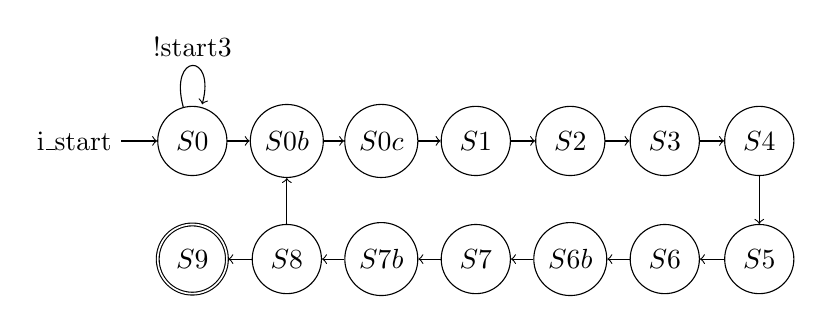
\begin{tikzpicture}
[->,align=center,node distance=1.2cm]
\node[state, initial, initial text=i\_start] (s0) {$S0$};
\node[state, right of=s0] (s0b) {$S0b$};
\node[state, right of=s0b] (s0c) {$S0c$};
\node[state, right of=s0c] (s1) {$S1$};
\node[state, right of=s1] (s2) {$S2$};
\node[state, right of=s2] (s3) {$S3$};
\node[state, right of=s3] (s4) {$S4$};
\node[state, below of=s4, node distance=1.5cm] (s5) {$S5$};
\node[state, left of=s5] (s6) {$S6$};
\node[state, left of=s6] (s6b) {$S6b$};
\node[state, left of=s6b] (s7) {$S7$};
\node[state, left of=s7] (s7b) {$S7b$};
\node[state, left of=s7b] (s8) {$S8$};
\node[state, accepting, left of=s8] (s9) {$S9$};
\draw   
	(s0) edge[loop above] node{!start3} (s0)
	(s0) edge[above] node{} (s0b)
	(s0b) edge[above] node{} (s0c)
	(s0c) edge[above] node{} (s1)
	(s1) edge[above] node{} (s2)
	(s2) edge[above] node{} (s3)
	(s3) edge[above] node{} (s4)
	(s4) edge[above] node{} (s5)
	(s5) edge[above] node{} (s6)
	(s6) edge[above] node{} (s6b)
	(s6b) edge[above] node{} (s7)
	(s7) edge[above] node{} (s7b)
	(s7b) edge[above] node{} (s8)
	(s8) edge[above] node{} (s9)
	(s8) edge[above] node{} (s0b);
	%(s0b) edge[loop above] node{} (s0b);
	%(s0b) edge[bend left, above] node{} (s0c)
	%(s0c) edge[bend left, below] node{} (s0b);
\end{tikzpicture}


\section{Risultati sperimentali}

Figures are an excellent mechanism for communicating many kinds of results. Great care should be taken to produce clear, well-constructed figures.When there are many related graphs or images, they should usually be combined into a single figure. 

Figures should be displayed near where they are first mentioned in the text and are numbered sequentially: Figure \ref{ex-fig} is an example. All figures and tables should be mentioned in the text.

It is best to send your figures in a {``}scalable{''} form such as Wolfram Mathematica Graphics Objects, Encapsulated PostScript (EPS) or PortableDocument Format (PDF). Figures can also be processed in {``}bitmap{''} formats such as BMP, PICT or TIFF, but scalable formats generally reproduce better.
Figures should reproduce well (i.e., without noticeable aliasing) on common printers. The source file for a particular figure must include all elements of the figure and should not require modification. Lettering should be consistent throughout a figure and must be no smaller than 6 points when the figure is at final size. Lines should be thick enough that they do not break up under reduction (single-pixel lines rarely suffice). Filled black areas must not drop out. Whenever possible, the figures should be oriented in the same sense as text (portrait mode). 
Computer programs or algorithm descriptions may be given either in equations or in figures. Literal expressions that occur as computer input or output should be given in typewriter font. 
Tables should include captions similar to those for figures and should be numbered sequentially throughout the paper: Table \ref{ex-table} is an example. Tables must be oriented with the text and use 9-point type, and should be enclosed by a box. 
\section{Simulazioni}
\label{main-text}
Risultati  dei  test  fatti  e  le ragioni di tali test -motivare le scelte
\begin{itemize}
\item TB Delta=255:

 input=[2,3,255,0,1,1,0,255]
 output=[255,0,1,1,0,255].    
    
   Il delta sarà massimo nel momento in cui \(MAXPixel = 255\) e \(MINPixel = 0\). Il valore del logaritmo è quindi massimo e lo \(shiftlevel=0\) (caso minimo) che porterà quindi ad avere in output gli stessi valori di input.
\item TB tutti 0 e tutti 255 \(Delta=0\):

 input=[2,3,0,0,0,0,0,0] 
 output=[0,0,0,0,0,0]
 
  input=[2,3,255,255,255,255,255,255] 
 output=[0,0,0,0,0,0]
 
 Il delta sarà nullo nel momento in cui tutti i valori dell'immagine saranno uguali. Sarà infatti MAXPixel=MINPixel, generando così uno \(shiftlevel=8\) (caso massimo) che porterà quindi ad avere in output solo valori nulli. Questo è anche intuitivamente immaginabile con una monocromia dell'immagine che quindi viene riportata al valore di default.
 \item TB con Shift massimo:
 
 input=[2,3,128,128,128,128,128,128] 
 output=[0,0,0,0,0,0]

Lo Shift sinistro di n posizioni equivale a moltiplicare \(Value*2^{n}\). Un caso importante da considerare è quando il valore di \(n=8\) : il valore di \(Current Pixel-MINPixel\) verrà quindi completamente portato a sinistra lasciando tutti zeri, rispetto alla rappresentazione di 8 bit del pixel. Questo è uno dei valori per cui \(Temp Pixel>255\) e si avrà quindi un output di valori massimi.
\item TB con Massimo e Minimo agli estremi di lettura : 
 
 input=[2,3,255,132,254,2,2,1] 
 output=[255,255,255,2,2,0]
 
 Potrebbe capitare la lettura non completa dell'input. Caso molto comune nei due estremi RAM(3) e RAM(\(COL*RIG+2\)), a volte non compresi nella ricerca del minimo e del massimo.
 
 \item TB con caso limite per LUT: 
 
  input=[2,3,200,199,170,177,180,171] 
 output=[255,2552,0,112,160,16]
 Delta=30 Shift=4
 
 input=[2,3,201,199,170,177,180,171] 
 output=[248,232,0,56,80,8]
 Delta=31 Shift=3
 
  Bisogna considerare che \(log (delta +1)\) risulta caso limite nel momento in cui il valore di delta assume valore \(2^{n}-1\) (con \(0<=n<=8\)). La LUT dell'implementazione, tiene già conto dell'argomento del logaritmo, cambiando quindi il valore ogni volta che viene raggiunto dal delta una potenza di \(2^{n}-1\).  
\end{itemize}
% Numbered lists of items are obtained with \begin{enumerate} ... \end{enumerate}
If a list of items is given in the text, such as: (\textit{a}) first item; (\textit{b})~second item; and so forth, they should be indicated with parenthesized letters in italic typeface.
\section{Risultati di sintesi}
%Consistent mathematical notation is essential to clear exposition. Try to use familiar notation; for example, avoid having \(x\)stand for an integer index.
% In LaTeX, such in-line equations are delimited by \(...\).
%
% For a full list of TeX symbols, see the LaTeX or TeX manuals.
% Boldface is obtained with \textbf{...}
% Roman (ordinary) font, often used for English words within equations,
% is obtained with \textrm{...} (note that spaces between words must be
% indicated explicitly).
Displayed equations that are referenced in the text should be numbered sequentially: 
% This is done automatically if the correct tags are used in LaTeX. 
\begin{equation}
e^{2\pi i}=1.
\label{exponential-equation}
\end{equation}

\begin{table}
\centerline{\small\begin{tabular}{|c|c|c|c|c|}
\hline
 \textbf{Site Type} & \textbf{Used} & \textbf{Fixed} & \textbf{Available} & \textbf{Util \%}\\
\hline
  Slice LUTs & 180 & 0 & 134600 & 0.13\\
\hline
  Slice Registers & 207 & 0 & 269200 & 0.08\\
\hline
	F7 Muxes & 0 & 0 & 67300 & 0.00\\
\hline
	F8 Muxes & 0 & 0 & 33650 & 0.00\\
\hline
\end{tabular}}
\caption{Utilization Design Information - Slice Logic}
\label{ex-table}
\end{table}

% Any text can be used in a \label to mark an equation. Usually it will 
% be a tag that relates to the content of the equation. 
Spaces should be inserted in equations where necessary to improve readability. Equations should be referred to as {``}equation (\ref{exponential-equation}).{''} Short equations may be inserted directly in the text, as in \(\beta =2\). Equations that involve extensive subscripts, superscripts or built-up objects should be displayed. Special symbols in equations must be strictly limited to those that can be produced with Wolfram Mathematica using common fonts.
If a formatting system other than Wolfram Mathematica or LaTeX is used, make sure that all symbols are very clearly identified, and that all subscripts and superscripts are evident. \textit{Complex Systems} allows many kinds of notation. It is suggested that symbols or words related to actual or theoretical computers be indicated in \texttt{typewriter font}. 
Great care should be taken in mixing plain English, mathematics and algorithm descriptions. Say, for example, {``}\(x\) is the position{''} rather than {``}\(x=\) position.{''} Consistency must be maintained between different occurrences of a symbol. If \(x\) is a mathematical symbol, make sure it appears as \(x\) everywhere, not sometimes as x or as \texttt{x}. As a rough guide, mathematical symbols should appear as \(x\) and computer symbols as \texttt{x}. 
\begin{theorem}
Theorems and other structured mathematical text should be used when it improves the presentation. They should not be a substitute for clear English exposition. 
\end{theorem}
\begin{proof}
Proofs can continue for several paragraphs. They should end with an empty square.
\end{proof}
\section{Conclusioni}
\section{About the References}
References should give pointers to background material and related work. They should record credit due to other authors. 
References are numbered sequentially throughout the text. 
% This is achieved automatically using \cite in LaTeX.
Each item should be given a separate number (except when citations are made to different portions of the same document: these should be indicated as {``}\cite[pp. 3--56]{text-a}{''} or {``}\cite[Chapter 14]{text-b}{''}). 
\textit{Full titles of papers should be given}. They should be enclosed in quotation marks, with all important words capitalized. Titles of printed items should be followed by a comma inside the quotation marks. Include the paper{'}s digital object identifier (DOI) name (number) if it is available(\url{www.doi.org/hb.html}). Titles accessible only via the internet are treated differently based on their type. See the examples described in the References section of this sample paper.
To cater to a wide variety of disciplines, it is important that \textit{all names of journals be spelled out in full} and italicized. (Use \textit{Physical ReviewLetters}, not\textit{ Phys. Rev. Lett.}, and \textit{Journal of Computer and System Science}, not \textit{J. Comput. Sys. Sci.}) 
For printed items, give the journal{'}s volume number in boldface (do not write the word {``}volume{''} explicitly). The issue number should be placed in parentheses immediately following the volume number, but not in bold: for example, \textbf{4}(1). Include months only when necessary, using their three-letter abbreviation. Give starting and ending page numbers.
Author names should be given with initials first, with spaces after each period. For sources that list more than 10 authors, the names of the first seven authors should be given, followed by {``}et al.{''} For sources with fewer than 10 authors, all names are listed.
Titles of books (i.e., published material with ISBN numbers) should be italicized. Names and cities of publishers and dates of publication should always be given. Conference proceedings that are distributed through ordinary publishers should be cited like books. 
Titles of proceedings and reports that are distributed in other ways or via the internet should be given in full in the standard roman typeface.URLs or other information on how to obtain them should be given following the title. Pricing information should not be included.
\section*{Acknowledgments}
Acknowledgments should thank individuals and organizations for their contributions to the work. All funding information should be placed in the acknowledgments.If acknowledgments imply some endorsement of the paper (e.g., {``}We thank X for checking\(\ldots\){''}), make sure the parties involved approve the statements made.
\begin{thebibliography}{99}
% The number of 9s indicate how many digits to allow for to align the indented list.
\bibitem{a-review}
% ``a-review'' is a sample tag: use a unique tag for each paper.
F. Authorlast and S. Authorlast, ``Article Title,'' \textit{Full
Name of Journal}, \textbf{volume}(issue number), year pp. \#--\#.
doi:name.\\
R. Albert and A.-L. Barab{\' a}si, ``Statistical Mechanics of Complex
Networks,'' \textit{Reviews of Modern Physics}, \textbf{74}(1), 
2002 pp. 47--97.  doi:10.1103/RevModPhys.74.47.
% Use \textit{...} for italics, \textbf{...} for boldface.
% Do not explicitly use the word ``volume''
% The full year (e.g., 1991) should be used for the date.
% Use -- to get an appropriate dash between page numbers.
\bibitem{text-a}
I. J. Authorlast, \textit{Book Title}, Publisher Location: Publisher Name, year. \\
T. C. Schelling, \textit{Micromotives and Macrobehavior}, New York: Norton, 1978. 
\bibitem{text-b}
A. Authorlast, ``Paper Title,'' in \textit{A Collection} (F. Editor and
S. Editor, eds.), Publisher Location: Publisher Name, year pp.
\#--\#. doi:name.\\
S. Hou, J. Sterling, S. Chen, and G. Doolen, ``A Lattice Boltzmann
Subgrid Model for High Reynolds Number Flows,'' in \textit{Pattern
Formation and Lattice Gas Automata} (A. T. Lawniczak and R. Kapral,
eds.), Toronto: Fields Institute Communications, \textbf{6}, 1996
pp. 151--166.
\bibitem{edbook}
A. Editor, ed., \textit{Book Title}, nth ed., Publisher Location: Publisher Name, year. \\
A. Law and D. Kelton, eds., \textit{Simulation Modeling and
Analysis}, 3rd ed., Boston: McGraw-Hill, 2000.
\bibitem{proc}
A. Authorlast, ``Paper Title,'' in \textit{Conference Proceedings
Title} (\textit{Conference Acronym and year}), Conference Location
(A. Authorlast, ed.), Publisher Location: Publisher Name, year pp.
\#--\#.\\
P. Fritzson, L. Viklund, J. Herber and D. Fritzson, ``Industrial
Application of Object-Oriented Mathematical Modeling and Computer
Algebra in Mechanical Analysis,'' in \textit{Proceedings of the
Seventh  International Conference on Technology of Object-Oriented
Languages and Systems (TOOLS EUROPE'92)}, Dortmund, Germany 
(G.  Heeg, B. Magnosson, and B. Meyer, eds.), Hertfordshire, UK: Prentice
Hall International (UK) Ltd., 1992 pp. 167--181.
\bibitem{report}
A. Authorlast, \textit{Technical Report Title}, Classification/Number,
Department, University or Organization, Location, year. URL if
available.\\
C. Lemieux, M. Cieslak, and K. Luttmer, \textit{RandQMC User's
Guide: A Package for Randomized Quasi-Monte Carlo Methods in C},
Technical report 2002-712-15, Department of Computer Science,
University of Calgary, 2002. hdl.handle.net/1880/46569.
\bibitem{preprint}
A. Authorlast, \textit{Preprint Book Title}, Publisher Location:
Publisher Name, forthcoming. \\
J.-P. Aubin, L. Chen, and O. Dordan, \textit{Tychastic Measure of
Viability Risk: A Viabilist Portfolio Performance and Insurance
Approach}, Heidelberg: Springer, forthcoming. 
vimades.com/AUBIN/EradicationVPPI-Presentation.pdf.
\bibitem{manual}
Company Name, \textit{Computer Program Reference Manual} (available from Name, address). \\
Xerox, \textit{InterLISP Reference Manual} (available from Xerox
Palo Alto Research Center, Palo Alto, CA).
\bibitem{future}
A. Authorlast, ``Future Paper,'' \textit{Full Name of Journal}, forthcoming.\\ 
J. Riedel and H. Zenil, ``Cross-Boundary Behavioural Reprogrammability Reveals Evidence of Pervasive Universality,'' \textit{ International Journal of Unconventional Computing}, forthcoming. arxiv.org/abs/1510.01671.
\bibitem{talk}
A. Authorlast, ``Title,'' presentation given at \textit{Conference
Name (Conference Acronym and year)}, Location. URL of abstract if
available.\\
A. Banos, ``Exploring Network Effects in Schelling's Segregation
Model,'' presentation given at \textit{S4-Modus Workshop: Multi-scale
Interactions between Urban Forms and Processes}, Besan{\c c}on,
France, 2009.
\bibitem{program}
Software Name, Release Version Number, Location: Organization, year.\\
U. Wilensky. ``NetLogo.'' Center for Connected Learning and
Computer-Based Modeling, Northwestern University, Evanston, IL.
(Oct 25, 2012) ccl.northwestern.edu/netlogo/index.shtml.
\bibitem{website}
A. Authorlast. ``Website (or page) Title.'' (Month Day, Year) URL.\\
OnlineAtlas.us. ``United States Interstate Highway Map.'' (May 7,
2012) www.onlineatlas.us/interstate-highways.htm.
\bibitem{blog}
A. Authorlast. ``Blog Title,'' Blog Series Name (blog). (Month Day, Year) URL.\\
B. Yorgey, ``Recounting the Rationals, Part II,'' \textit{The Math
Less Traveled} (blog). (Apr 2, 2010) www.mathlesstraveled.com/?p=97.
\bibitem{forum}
A. Authorlast. ``Forum Post'' from Forum Name. (Month Day, Year) URL.\\
T. Rowland. ``Enumerating Strings'' from The NKS Forum---A
Wolfram Web Resource. (Apr 02, 2010)\\
forum.wolframscience.com/showthread.php?s=$\&$threadid=929.
\bibitem{demonstration}
A. Authorlast. ``Demonstration Title'' from the Wolfram Demonstrations
Project---A Wolfram Web Resource. URL.\\
E. Pegg Jr. ``Coin Flips'' from the Wolfram Demonstrations Project---A
Wolfram Web Resource. www.demonstrations.wolfram.com/CoinFlips.
\bibitem{cloud}
A. Authorlast. ``Wolfram Cloud Article Title.'' (Month Day, Year) URL.\\
A. A. de Laix. ``Encryption with Enigma.'' (Jul 1, 2014) www.wolframcloud.com/objects/1f52ae4b-0686-4bde-966e-5e60d8225ae4.
\end{thebibliography}
\end{document}